The experiments we have discussed so far are fairly simple. They have
one independent variable with two levels, and a single dependent
variable. Experiments can become much more complicated by adding more
levels to the independent variable, adding more independent variables,
and/or adding more dependent variables. As experiments become more
complicated, the basic empirical question remains the same: Did the
manipulation(s) cause change in the measure(s). To ease into more
complex designs we will discuss single factor designs with more than two
levels.

\subsection{Quantitative vs.~Qualitative Independent
variables}\label{quantitative-vs.qualitative-independent-variables}

A single factor design with more than two levels involves a single
independent variable (factor), and typically a single dependent
variable. Importantly, the independent variable has more than two
levels. Two common kinds of multi-level designs involve either
quantitative or qualititative manipulations of the independent variable.

\begin{figure}
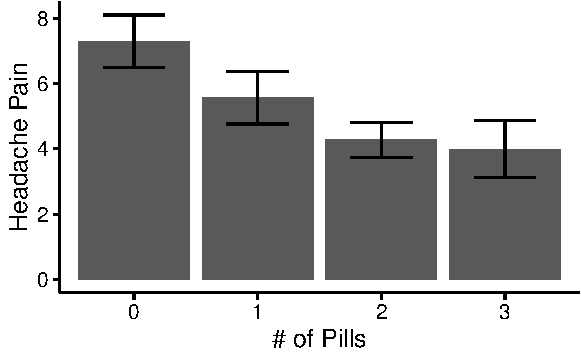
\includegraphics[width=.6\linewidth]{OneWay_files/figure-latex/unnamed-chunk-1-1} 
\end{figure}

A quantitative manipulation is a change in magnitude, or amount. For
example, a drug company might be interested in testing not only whether
or not Drug A reduces headache (perhaps by comparing one group that gets
the drug, and another that does not), but also how the amount of the
drug influences reductions in headache pain. So, a multi-level
experiment might have a few groups who receive, 0, 1, 2, 3, 4 or more
pills, respectively.

\begin{figure}
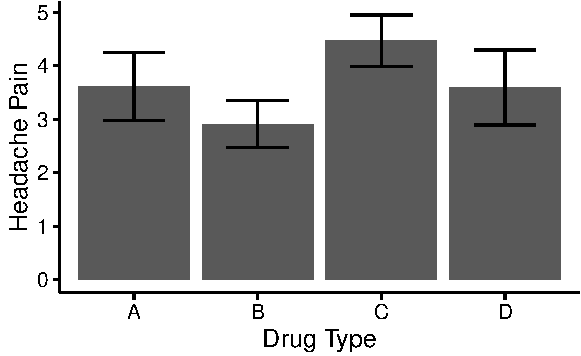
\includegraphics[width=.6\linewidth]{OneWay_files/figure-latex/unnamed-chunk-2-1} \end{figure}

A qualitative manipulation involves categorically different conditions.
For example, a drug company might be interested in comparing the
relative effectiveness of different kinds of drugs in reducing headache
pain. They could conduct a multi-level experiment with each group
receiving a different drug, drug A, drug B, drug C, and so on.

\subsection{Interpreting the pattern of results}\label{interpreting-the-pattern-of-results}

\begin{marginfigure}
Possible patterns of differences between means in a design with three
levels

\begin{enumerate}
\def\labelenumi{\arabic{enumi}.}
\item
  A = B = C
\item
  A = B \textgreater{} C
\item
  A = B \textless{} C
\item
  A \textgreater{} B = C
\item
  A \textless{} B = C
\item
  A \textless{} B \textless{} C
\item
  A \textgreater{} B \textgreater{} C
\item
  A = C \textgreater{} B
\item
  A = C \textless{} B
\end{enumerate}
\end{marginfigure}

Designs with only two levels are fairly straightforward to interpret
because there are only a few possible kinds of patterns of differences
that can be observed. These include: A\textgreater{}B, A=B, and
A\textless{}B. Or even more simply: A is the same as B (A=B), or A is
not the same as B (A\textgreater{}B, or A\textless{}B).

The number of possible patterns that could be observed increases with
each additional level. For example, consider an experiment with three
levels A, B, and C. The possible patterns that could be observed are
shown on the right.

As with two level designs, when reporting the results of experiments
with multiple levels, it is very important to explain the pattern of
means across conditions. This involves telling the reader which means
were different from one another, and which means were the same.

Again, as with 2-level designs, the process of random sampling can
produce differences in the sample means for each of the levels. So,
researchers also conduct statistical tests to determine the likelihood
that the results that they observed could have been obtained by chance
alone. The most common statistical test used in this case is the one-way
ANOVA (Analysis of Variance). The chapter on inferential statistics goes
into more detail about ANOVAs, and we assume that you have some memories
of how ANOVAs work from your statistics class. Nevertheless, we go
through an example to illustrate the basic process. Note, this example
is the same one discussed in chapter four of your lab manual.

\subsection{An example one-way ANOVA using
R}\label{an-example-one-way-anova-using-r}

Consider an experiment where subjects attempt to memorize words for a
later recall test under five different conditions. This will be a
between-subjects experiment with 10 simulated subjects in each
condition. We will have condition A, B, C, D, and E. For example,
condition A could be repeating each word silently to yourself, condition
B could be creating a mental picture of each word, and so on. To
simulate data for each subject we need to make some assumptions. Let's
say that out of 30 words most people remember about 15 of them, but
there is variation, so some people do better and some people do worse.
We can model this by sampling numbers randomly from a distribution of
our choice. For convenience, we will use the normal distribution. Let's
imagine that condition A and B help memory more than C and D, and that
memory is worse in condition E. Here is the R code and output for
simulating this kind of data.

\begin{Shaded}
\begin{Highlighting}[]
\NormalTok{A<-}\KeywordTok{round}\NormalTok{(}\KeywordTok{rnorm}\NormalTok{(}\DecValTok{10}\NormalTok{,}\DecValTok{20}\NormalTok{,}\DecValTok{2}\NormalTok{))}
\NormalTok{B<-}\KeywordTok{round}\NormalTok{(}\KeywordTok{rnorm}\NormalTok{(}\DecValTok{10}\NormalTok{,}\DecValTok{20}\NormalTok{,}\DecValTok{2}\NormalTok{))}
\NormalTok{C<-}\KeywordTok{round}\NormalTok{(}\KeywordTok{rnorm}\NormalTok{(}\DecValTok{10}\NormalTok{,}\DecValTok{15}\NormalTok{,}\DecValTok{2}\NormalTok{))}
\NormalTok{D<-}\KeywordTok{round}\NormalTok{(}\KeywordTok{rnorm}\NormalTok{(}\DecValTok{10}\NormalTok{,}\DecValTok{15}\NormalTok{,}\DecValTok{2}\NormalTok{))}
\NormalTok{E<-}\KeywordTok{round}\NormalTok{(}\KeywordTok{rnorm}\NormalTok{(}\DecValTok{10}\NormalTok{,}\DecValTok{10}\NormalTok{,}\DecValTok{2}\NormalTok{))}
\NormalTok{all_data<-}\KeywordTok{data.frame}\NormalTok{(A,B,C,D,E)}
\KeywordTok{kable}\NormalTok{(all_data,}\DataTypeTok{format=}\StringTok{"latex"}\NormalTok{)}
\end{Highlighting}
\end{Shaded}

\begin{tabular}{r|r|r|r|r}
\hline
A & B & C & D & E\\
\hline
18 & 22 & 17 & 16 & 9\\
\hline
22 & 18 & 13 & 15 & 11\\
\hline
16 & 20 & 15 & 12 & 7\\
\hline
22 & 22 & 16 & 14 & 7\\
\hline
17 & 20 & 18 & 18 & 13\\
\hline
19 & 21 & 18 & 17 & 9\\
\hline
20 & 19 & 14 & 13 & 15\\
\hline
21 & 18 & 15 & 13 & 10\\
\hline
19 & 19 & 13 & 14 & 9\\
\hline
22 & 22 & 17 & 16 & 10\\
\hline
\end{tabular}

We have produced a table with fake data for 10 subjects in each
condition. The numbers all represent the number of correctly recalled
words for each simulated subject. For groups A and B we sample 10
numbers, from a distribution with mean 20, and standard deviation 2.
This is a higher mean than groups C and D (mean = 15). The lowest mean
was for Group E (mean = 10). So, on average, groups A and B should have
higher scores than C and D, which should be higher than E.

Ok, so what happened in our simulated experiment. We can see the numbers
in the table, but it would be nice to summarize them so we can more
easily look at differences. After all, it's hard to make sense of a
bunch of raw data in a table.

One way to summarize the data is to compute the group means for each
condition. This averages over the subjects, and gives us only 5 means to
look at, so it is easier to see the differences. We can ``easily'' do
this in R in a couple different ways. However, R often likes the data in
a particular format, in this case long-data format. So, we will first
convert to that format, and see what it looks like.

\begin{Shaded}
\begin{Highlighting}[]
\NormalTok{long_data<-}\KeywordTok{data.frame}\NormalTok{(}\DataTypeTok{Conditions=}\KeywordTok{rep}\NormalTok{(}\KeywordTok{c}\NormalTok{(}\StringTok{"A"}\NormalTok{,}\StringTok{"B"}\NormalTok{,}\StringTok{"C"}\NormalTok{,}\StringTok{"D"}\NormalTok{,}\StringTok{"E"}\NormalTok{),}\DataTypeTok{each=}\DecValTok{10}\NormalTok{),}
                      \DataTypeTok{Recall=}\KeywordTok{c}\NormalTok{(A,B,C,D,E))}
\KeywordTok{kable}\NormalTok{(long_data[}\DecValTok{1}\NormalTok{:}\DecValTok{25}\NormalTok{,],}\DataTypeTok{format=}\StringTok{"latex"}\NormalTok{)}
\end{Highlighting}
\end{Shaded}

\begin{tabular}{l|r}
\hline
Conditions & Recall\\
\hline
A & 18\\
\hline
A & 22\\
\hline
A & 16\\
\hline
A & 22\\
\hline
A & 17\\
\hline
A & 19\\
\hline
A & 20\\
\hline
A & 21\\
\hline
A & 19\\
\hline
A & 22\\
\hline
B & 22\\
\hline
B & 18\\
\hline
B & 20\\
\hline
B & 22\\
\hline
B & 20\\
\hline
B & 21\\
\hline
B & 19\\
\hline
B & 18\\
\hline
B & 19\\
\hline
B & 22\\
\hline
C & 17\\
\hline
C & 13\\
\hline
C & 15\\
\hline
C & 16\\
\hline
C & 18\\
\hline
\end{tabular}

I've only printed the first 25 lines, but the dataframe contains all of
the data for conditions, C, D, and E as well. You can see why they call
it long format. It's because each data point gets it's own row in the
table.

\subsection{Looking at the means}\label{looking-at-the-means}

Now that the data is in long format we can easily make a table of the
condition means

\begin{Shaded}
\begin{Highlighting}[]
\NormalTok{condition_means<-}\KeywordTok{aggregate}\NormalTok{(Recall~Conditions,long_data,mean)}
\KeywordTok{kable}\NormalTok{(condition_means,}\DataTypeTok{format=}\StringTok{"latex"}\NormalTok{)}
\end{Highlighting}
\end{Shaded}

\begin{tabular}{l|r}
\hline
Conditions & Recall\\
\hline
A & 19.6\\
\hline
B & 20.1\\
\hline
C & 15.6\\
\hline
D & 14.8\\
\hline
E & 10.0\\
\hline
\end{tabular}

We can now see the group means, but we can't see any measure of how
variable the data are in each condition. We might, for example, also
want to compute the standard deviation as well as the mean, and put them
both in the table. We could run the same code from above and substite sd
for mean, which would give us a table of standard deviations. However,
we will use a more advanced function from the plyr package, called
ddply. ddply let's you compute multiple statistics and put them all in a
single table. The syntax is a bit different, but it doesn't take long to
get used to it.

\begin{Shaded}
\begin{Highlighting}[]
\KeywordTok{library}\NormalTok{(plyr)}
\NormalTok{condition_means<-}\KeywordTok{ddply}\NormalTok{(long_data,.(Conditions),summarise,}
                       \DataTypeTok{MeanRecall=}\KeywordTok{mean}\NormalTok{(Recall),}
                       \DataTypeTok{StdDeviation=}\KeywordTok{sd}\NormalTok{(Recall))}
\KeywordTok{kable}\NormalTok{(condition_means,}\DataTypeTok{format=}\StringTok{"latex"}\NormalTok{)}
\end{Highlighting}
\end{Shaded}

\begin{tabular}{l|r|r}
\hline
Conditions & MeanRecall & StdDeviation\\
\hline
A & 19.6 & 2.170509\\
\hline
B & 20.1 & 1.595131\\
\hline
C & 15.6 & 1.897367\\
\hline
D & 14.8 & 1.932184\\
\hline
E & 10.0 & 2.494438\\
\hline
\end{tabular}

\subsection{Plotting the data}\label{plotting-the-data}

It's often very desirable to plot the data in a graph, rather than just
present the means in a table. People find it easier to look at graphs,
because the differences in the data just pop-out much easier than
looking at numbers in a table. R has a fantastic graphing package called
ggplot2. ggplot2 is a whole philosophy for visual design and
data-presentation, and it can be daunting at first. But, it's complexity
makes it very powerful, and when you get the hang of it you can very
quickly make all sorts of beautiful graphs to present data. Here is some
code to make ggplot create a bar graph to plot the means, along with
error bars. In this case the error bars with represent standard errors
of the mean, rather than standard deviations. R does not have a built in
function for the standard error of the mean, so we have to write it
ourselves.

\begin{Shaded}
\begin{Highlighting}[]
\KeywordTok{library}\NormalTok{(ggplot2)}
\NormalTok{sde<-function(x)\{}\KeywordTok{sd}\NormalTok{(x)/}\KeywordTok{length}\NormalTok{(x)\}}
\NormalTok{plot_means<-}\KeywordTok{ddply}\NormalTok{(long_data,.(Conditions),summarise,}
                       \DataTypeTok{MeanRecall=}\KeywordTok{mean}\NormalTok{(Recall),}
                       \DataTypeTok{SE=}\KeywordTok{sde}\NormalTok{(Recall))}

\NormalTok{limits <-}\StringTok{ }\KeywordTok{aes}\NormalTok{(}\DataTypeTok{ymax =} \NormalTok{MeanRecall +}\StringTok{ }\NormalTok{SE, }\DataTypeTok{ymin =} \NormalTok{MeanRecall -}\StringTok{ }\NormalTok{SE)}

\KeywordTok{ggplot}\NormalTok{(plot_means,}\KeywordTok{aes}\NormalTok{(}\DataTypeTok{x=}\NormalTok{Conditions, }\DataTypeTok{y=}\NormalTok{MeanRecall))+}
\StringTok{  }\KeywordTok{geom_bar}\NormalTok{(}\DataTypeTok{position=}\StringTok{"dodge"}\NormalTok{,}\DataTypeTok{stat=}\StringTok{"identity"}\NormalTok{)+}
\StringTok{  }\KeywordTok{geom_errorbar}\NormalTok{(limits, }\DataTypeTok{width=}\NormalTok{.}\DecValTok{1}\NormalTok{)+}
\StringTok{  }\KeywordTok{theme_classic}\NormalTok{(}\DataTypeTok{base_size=}\DecValTok{12}\NormalTok{)+}
\StringTok{  }\KeywordTok{ylab}\NormalTok{(}\StringTok{"Mean Correctly }\CharTok{\textbackslash{}n}\StringTok{ Recalled Words"}\NormalTok{)+}
\StringTok{  }\KeywordTok{xlab}\NormalTok{(}\StringTok{"Condition"}\NormalTok{)}
\end{Highlighting}
\end{Shaded}

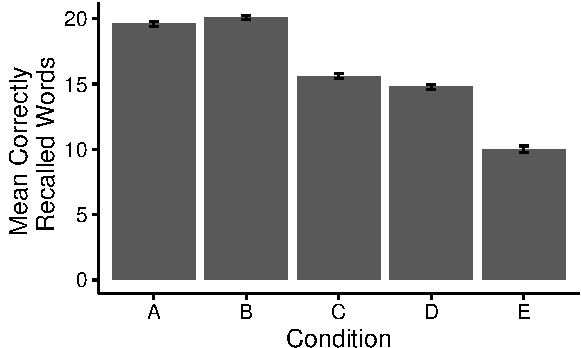
\includegraphics{OneWay_files/figure-latex/unnamed-chunk-8-1}

Now it is easy to the differences between conditions. Just as we had
hoped, Groups A and B appear to have recalled more words than Groups C
and D, which remembered more words than group E.

\subsection{Conducting the ANOVA}\label{conducting-the-anova}

Although the graph and the tabe show some clear differences in the
means, we still want to find out the probability that this kind of
finding occurs by chance alone. We can be confident in the differences
when we know that they do not occur very often by chance alone. The
first step is conduct a one-way ANOVA. This is very easy in R.

\begin{Shaded}
\begin{Highlighting}[]
\NormalTok{aov.out<-}\KeywordTok{aov}\NormalTok{(Recall~Conditions,long_data)}
\end{Highlighting}
\end{Shaded}

We're done! It's only one line of code. However, we need a couple more
to see the results.

\begin{Shaded}
\begin{Highlighting}[]
\NormalTok{aov_summary<-}\KeywordTok{summary}\NormalTok{(aov.out)}
\KeywordTok{kable}\NormalTok{(}\KeywordTok{xtable}\NormalTok{(aov_summary),}\DataTypeTok{format=}\StringTok{"latex"}\NormalTok{)}
\end{Highlighting}
\end{Shaded}

\begin{tabular}{l|r|r|r|r|r}
\hline
  & Df & Sum Sq & Mean Sq & F value & Pr(>F)\\
\hline
Conditions & 4 & 673.68 & 168.420000 & 40.46396 & 0\\
\hline
Residuals & 45 & 187.30 & 4.162222 & NA & NA\\
\hline
\end{tabular}

The ANOVA table gives us a bunch of information. We will go into much
greater detail about the meaning of each number in the table, but also
assume for now that you are somewhat familiar with these ideas because
you have already taken statistics, right?

We are mainly interested in the p-value, which tells how often results
like the ones we found can occur by chance. But, when we report the
results of our ANOVA, we also provide additional information about the
F-value, the degrees of freedom values, and the mean squared error term.
The reason is that if you know these numbers, you can actually
reconstruct all of the other numbers. The results of our ANOVA are
significant. You could report this in a sentence like the following.

The main effect of condition was significant, F(4, 45) = 40.46, MSE =
4.16, p \textless{} .001.

\subsection{Comparisons between
conditions}\label{comparisons-between-conditions}

The p-value from above is much smaller than .05, which shows the
difference between conditions in the data does not occur very often by
chance alone. However, because we conducted an omni-bus test, we only
know that there is some difference between conditions, but we do not
know which specific conditions are different from one another.

So, we have to conduct additional tests between specific conditions.
There are multiple strategies for conducting these tests. For now, we
will simply run t-tests between comparisons of interest.

Remember, our data simulated the pattern that memory recall would be
better for groups A and B, which would be better than groups C and D,
which would better than group E. In other words A=B \textgreater{} C=D
\textgreater{} E.

We can confirm this pattern by conducting tests to see if it holds up.
For example, how would we test the pattern A=B \textgreater{} C=D
\textgreater{} E, all of the following comparisons need to be true,

\begin{itemize}
\item
  A = B
\item
  A \textgreater{} C
\item
  A \textgreater{} D
\item
  B \textgreater{} C
\item
  B \textgreater{} D
\item
  C = D
\end{itemize}

and, all of the conditions should be greater than E

\begin{itemize}
\item
  A \textgreater{} E
\item
  B \textgreater{} E
\item
  C \textgreater{} E
\item
  D \textgreater{} E
\end{itemize}

Let's conduct a few of these tests, and then report the findings.

\begin{Shaded}
\begin{Highlighting}[]
\KeywordTok{library}\NormalTok{(broom)}
\CommentTok{#conduct t-tests}
\NormalTok{ab<-}\KeywordTok{tidy}\NormalTok{(}\KeywordTok{t.test}\NormalTok{(A,B,}\DataTypeTok{var.equal =} \OtherTok{TRUE}\NormalTok{))}
\NormalTok{ac<-}\KeywordTok{tidy}\NormalTok{(}\KeywordTok{t.test}\NormalTok{(A,C,}\DataTypeTok{var.equal =} \OtherTok{TRUE}\NormalTok{))}
\NormalTok{cd<-}\KeywordTok{tidy}\NormalTok{(}\KeywordTok{t.test}\NormalTok{(C,D,}\DataTypeTok{var.equal =} \OtherTok{TRUE}\NormalTok{))}
\NormalTok{de<-}\KeywordTok{tidy}\NormalTok{(}\KeywordTok{t.test}\NormalTok{(D,E,}\DataTypeTok{var.equal =} \OtherTok{TRUE}\NormalTok{))}

\CommentTok{#put the results in a table}
\NormalTok{alltests<-}\KeywordTok{rbind}\NormalTok{(ab,ac,cd,de)}
\NormalTok{alltests<-}\KeywordTok{cbind}\NormalTok{(alltests,}\DataTypeTok{Comparison=}\KeywordTok{c}\NormalTok{(}\StringTok{"AB"}\NormalTok{,}\StringTok{"AC"}\NormalTok{,}\StringTok{"CD"}\NormalTok{,}\StringTok{"DE"}\NormalTok{))}
\NormalTok{finaltable <-}\StringTok{ }\KeywordTok{subset}\NormalTok{(alltests, }\DataTypeTok{select =} \KeywordTok{c}\NormalTok{(Comparison,estimate1,estimate2,statistic,p.value,parameter))}
\KeywordTok{kable}\NormalTok{(finaltable,}\DataTypeTok{format=}\StringTok{"latex"}\NormalTok{)}
\end{Highlighting}
\end{Shaded}

\begin{tabular}{l|r|r|r|r|r}
\hline
Comparison & estimate1 & estimate2 & statistic & p.value & parameter\\
\hline
AB & 19.6 & 20.1 & -0.5869954 & 0.5644975 & 18\\
\hline
AC & 19.6 & 15.6 & 4.3876345 & 0.0003550 & 18\\
\hline
CD & 15.6 & 14.8 & 0.9341987 & 0.3625653 & 18\\
\hline
DE & 14.8 & 10.0 & 4.8107024 & 0.0001401 & 18\\
\hline
\end{tabular}

\subsection{Writing it all up}\label{writing-it-all-up}

The following is an example results section for our hypothetical
experiment. This could serve as a model for your own results section.

The number of correctly recalled words for each subject in each
condition were submitted to a one-way ANOVA, with memorization condition
(A, B, C, D, and E) as the sole between-subjects factor. Mean recall
scores in each condition are displayed in Figure 1.

The main effect of memorization condition was significant, F(4, 45) =
40.46, MSE = 4.16, p \textless{} .001. Figure 1 shows that Groups A and
B had higher recall scores than Groups C and D, which had higher recall
scores than Group E. This pattern was confirmed across four independent
sample t-tests. Group A (M = 19.6) and Group B (M = 20.1) were not
significantly different t(18) = -0.59, p =0.564. Group A recalled
significantly more words than Group C (M = 15.6), t(18) = 4.39, p =0.
Group C and Group D (M = 14.8) were not significantly different t(18) =
0.93, p =0.363. Finally, Group D recalled significantly more words than
Group E (M = 10), t(18) = 4.81, p =0.

